%%%%%%%%%%%%%%%%%%%%%%%%%%%%%%%%%%%%%
%                                   %
% Compile with XeLaTeX and biber    %
%                                   %
% Questions or comments:            %
%                                   %
% joshua dot mcneill at uga dot edu %
%                                   %
%%%%%%%%%%%%%%%%%%%%%%%%%%%%%%%%%%%%%

\documentclass{beamer}
  % Read in standard preamble (cosmetic stuff)
  %%%%%%%%%%%%%%%%%%%%%%%%%%%%%%%%%%%%%%%%%%%%%%%%%%%%%%%%%%%%%%%%
% This is a standard preamble used in for all slide documents. %
% It basically contains cosmetic settings.                     %
%                                                              %
% Joshua McNeill                                               %
% joshua dot mcneill at uga dot edu                            %
%%%%%%%%%%%%%%%%%%%%%%%%%%%%%%%%%%%%%%%%%%%%%%%%%%%%%%%%%%%%%%%%

% Beamer settings
% \usetheme{Berkeley}
\usetheme{CambridgeUS}
% \usecolortheme{dove}
% \usecolortheme{rose}
\usecolortheme{seagull}
\usefonttheme{professionalfonts}
\usefonttheme{serif}
\setbeamertemplate{bibliography item}{}

% Packages and settings
\usepackage{fontspec}
  \setmainfont{Charis SIL}
\usepackage{hyperref}
  \hypersetup{colorlinks=true,
              allcolors=blue}
\usepackage{graphicx}
  \graphicspath{{../../figures/}}
\usepackage[normalem]{ulem}
\usepackage{enumerate}

% Document information
\author{M. McNeill}
\title[FREN2001]{Français 2001}
\institute{\url{joshua.mcneill@uga.edu}}
\date{}

%% Custom commands
% Lexical items
\newcommand{\lexi}[1]{\textit{#1}}
% Gloss
\newcommand{\gloss}[1]{`#1'}
\newcommand{\tinygloss}[1]{{\tiny`#1'}}
% Orthographic representations
\newcommand{\orth}[1]{$\langle$#1$\rangle$}
% Utterances (pragmatics)
\newcommand{\uttr}[1]{`#1'}
% Sentences (pragmatics)
\newcommand{\sent}[1]{\textit{#1}}
% Base dir for definitions
\newcommand{\defs}{../definitions}


  % Packages and settings
  \usepackage[backend=biber, style=apa]{biblatex}
    \addbibresource{../references/References.bib}

  % Document information
  \subtitle[Psycholinguistics Intro]{Introduction to Psycholinguistics}

  %% Custom commands
  % Subsection/frame titles
  \newcommand{\suboneone}{What is it?}
  \newcommand{\subtwoone}{A little anatomy}
  \newcommand{\subtwotwo}{Language centers}
  \newcommand{\subtwothree}{Disorders}
  \newcommand{\subtwofour}{Practice}

\begin{document}
  % Read in the standard intro slides (title page and table of contents)
  %%%%%%%%%%%%%%%%%%%%%%%%%%%%%%%%%%%%%%%%%%%%%%%%%%%%%%%%%%%%%%%%
% This is a standard set of intro slides used in for all slide %
% documents. It basically contains the title page and table of %
% contents.                                                    %
%                                                              %
% Joshua McNeill                                               %
% joshua dot mcneill at uga dot edu                            %
%%%%%%%%%%%%%%%%%%%%%%%%%%%%%%%%%%%%%%%%%%%%%%%%%%%%%%%%%%%%%%%%

\begin{frame}
  \titlepage
  \tiny{Office: % Basically a variable for office hours location
Gilbert 121\\
        Office hours: % Basically a variable for office hours
 lundi, mercredi, vendredi 10:10--11:10
}
\end{frame}

\begin{frame}
  \tableofcontents[hideallsubsections]
\end{frame}

\AtBeginSection[]{
  \begin{frame}
    \tableofcontents[currentsection,
                     hideallsubsections]
  \end{frame}
}


  \section{Psycholinguistics}
    \subsection{\suboneone}
      \begin{frame}{\suboneone}
        \begin{block}{Theoretical linguists use deductive reasoning}
          \begin{itemize}
            \item Phonology (but not phonetics)
            \item Morphology
            \item Syntax
            \item Semantics (but not pragmatics)
          \end{itemize}
        \end{block}
        \begin{block}{Psycholinguists use inductive reasoning}
          i.e., Experimentation
        \end{block}
      \end{frame}

      \begin{frame}{\suboneone}
        \begin{alertblock}{Psycholinguistics}
          % Psycholinguistics
The study of how the mind processes, learns, stores, and produces language

        \end{alertblock}
        \begin{block}{The related field of \alert{neurolinguistics}}
          % Neurolinguistics
The study of the neural mechanisms involved in processing, learning, storing, and producing language

        \end{block}
      \end{frame}

  \section{The Brain}
    \subsection{\subtwoone}
      \begin{frame}[t]{\subtwoone}
        \begin{center}
          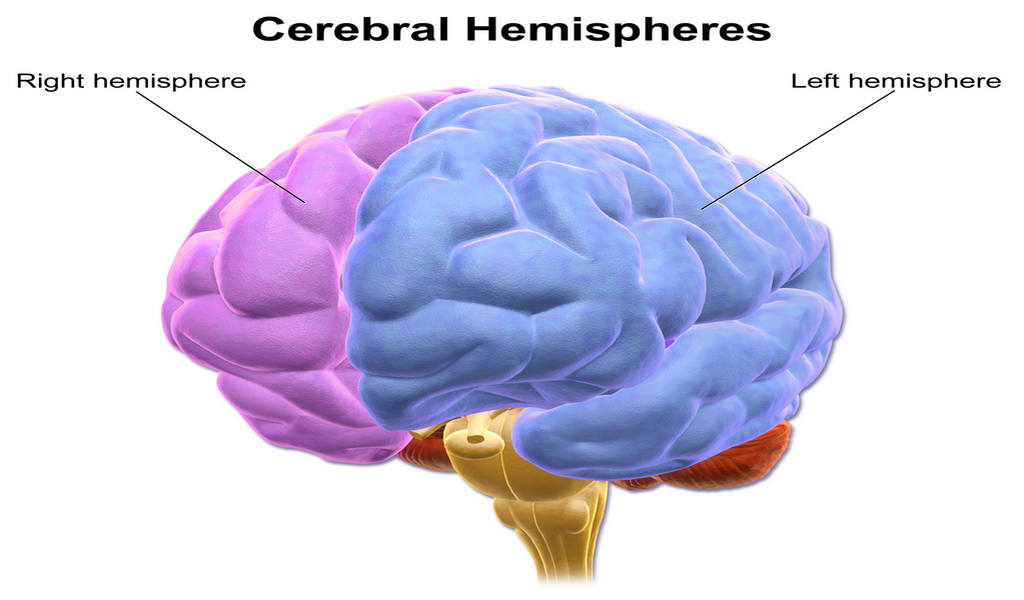
\includegraphics[scale=0.175]{cerebral_hemispheres.jpg}
        \end{center}
        \only<1>{
          \begin{alertblock}{Cerebrum}
            % Cerebrum
The largest part of the brain, whose cortex is responsible for most cognitive functions

          \end{alertblock}
        }
        \only<2>{
          \begin{alertblock}{Cerebral cortex}
            % Cerebral cortex
The outter layer of the cerebrum, which is responsible for most cognitive functions

            \begin{itemize}
              \item Location of the language centers
            \end{itemize}
          \end{alertblock}
        }
        \only<3>{
          \begin{block}{}
            The two hemispheres and the \alert{corpus callosum}:
            \begin{itemize}
              \item % Corpus callosum
The roughly 200 million neural fibers connecting the two hemispheres of the cerebrum, allowing them to communicate

            \end{itemize}
          \end{block}
        }
      \end{frame}

      \begin{frame}[t]{\subtwoone}
        \begin{center}
          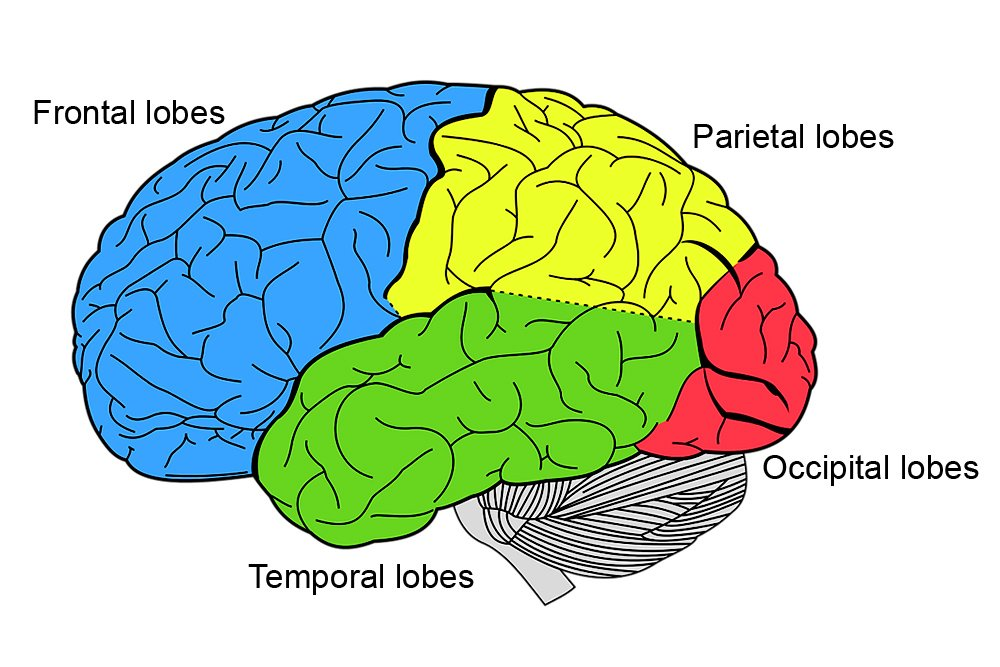
\includegraphics[scale=0.14]{cerebral_lobes.jpg}
        \end{center}
        \only<1-2>{
          \begin{block}{Four lobes}
            \begin{itemize}
              \item Occipital\uncover<2->{: Handles visual processing}
              \item Parietal\uncover<2->{: Handles tactile processing}
              \item \alert<2->{Temporal}
              \item \alert<2->{Frontal}
            \end{itemize}
          \end{block}
        }
        \only<3>{
          \begin{alertblock}{Temporal lobe}
            % Temporal lobe
The part of the cerebrum responsible for auditory processing

          \end{alertblock}
        }
        \only<4>{
          \begin{alertblock}{Frontal lobe}
            % Frontal lobe
The part of the cerebrum responsible for higher thinking and language production

          \end{alertblock}
        }
        \only<5>{
          \begin{block}{The bumps and grooves}
            \begin{itemize}
              \item \alert{Fissure}: % Fissure
A groove in the brain the divides it into lobes

              \item \alert{Gyrus}: % Gyrus
A ridge in the brain

              \item \alert{Sulcus}: % Sulcus
A groove in the brain the divides it into gyri

            \end{itemize}
          \end{block}
        }
        \only<6>{
          \begin{block}{To describe a location}
            hemisphere $+$ direction $+$ lobe $+$ gyrus/sulcus
            \begin{itemize}
              \item We will only need the directions \emph{superior} and \emph{inferior}
            \end{itemize}
          \end{block}
        }
        \only<7->{
          \begin{example}
            Left inferior frontal gyrus (LIFG)
            \begin{itemize}
              \item<8-> This is Broca's area
            \end{itemize}
          \end{example}
        }
      \end{frame}

    \subsection{\subtwotwo}
      \begin{frame}{\subtwotwo}
        \begin{alertblock}{Lateralization}
          % Lateralization
The tendency for some cognitive functions to be specialized to one hemisphere of the cerebrum or the other

        \end{alertblock}
        \begin{block}<2->{}
          The language centers are lateralized left for 96\% of right-handers and 73\% of left-handers \parencite{knecht_handedness_2000}
          \begin{itemize}
            \item We'll assume this for our descriptions here
          \end{itemize}
        \end{block}
        \begin{block}<3->{Disclaimer}
          Rapidly advancing area of research; subject to change
        \end{block}
      \end{frame}

      \begin{frame}{\subtwotwo}
        \begin{block}{}
          In the frontal lobe:
          \begin{itemize}
            \item Left inferior frontal gyrus (LIFG)
          \end{itemize}
          In the temporal lobe:

          \begin{minipage}[t]{0.48\linewidth}
            \begin{itemize}
              \item Left superior temporal gyrus (LSTG)
              \item Left inferior temporal gyrus (LITG)
            \end{itemize}
          \end{minipage}
          \begin{minipage}[t]{0.48\linewidth}
            \begin{itemize}
              \item Left parietotemporal junction (LPTJ)
              \item Angular gyrus
            \end{itemize}
          \end{minipage}
        \end{block}
      \end{frame}

      \begin{frame}[t]{\subtwotwo}
        \begin{center}
          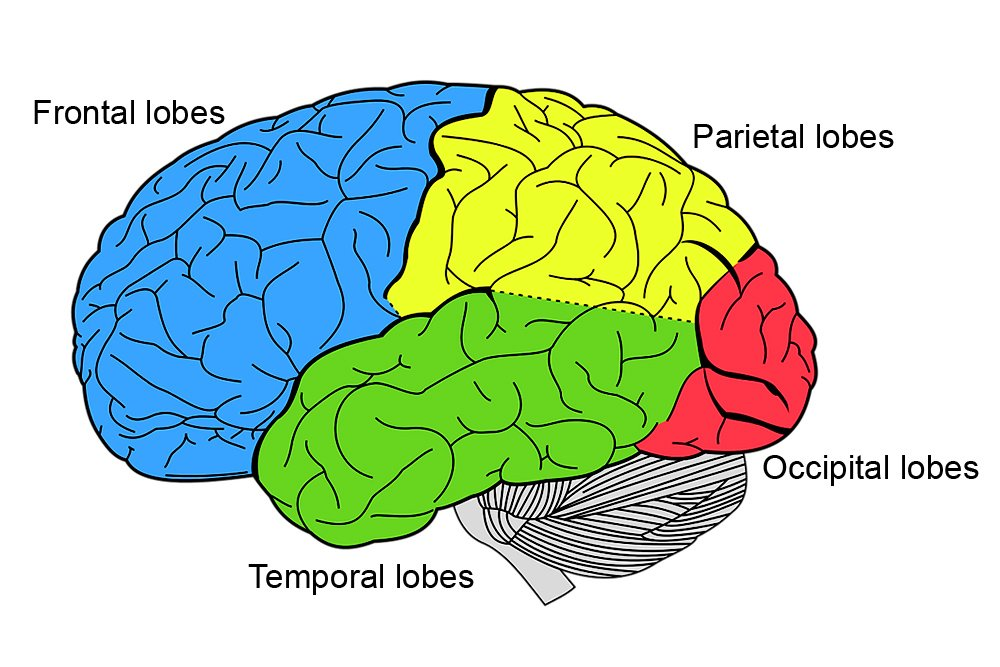
\includegraphics[scale=0.14]{cerebral_lobes.jpg}
        \end{center}
        \only<1>{
          \begin{block}{LIFG, aka \alert{Broca's area}}
            % Broca's area
The area of the cerebral cortex responsible for articulation and syntax

          \end{block}
        }
        \only<2>{
          \begin{block}{LSTG, aka \alert{Wernicke's area}}
            % Wernicke's area
The area of the cerebral cortex responsible for integrated syntax with morphology and semantics, traditionally thought to simply be responsible for comprehension

          \end{block}
        }
        \only<3>{
          \begin{block}{LITG}
            Responsible for \emph{lexical} semantics
          \end{block}
        }
        \only<4>{
          \begin{block}{LPTJ or the Sylvian fissure}
            Responsible for linking phonological representations to articulatory-motor representations
          \end{block}
        }
        \only<5>{
          \begin{block}{Angular gyrus, between the LPTJ and LSTG}
            Responsible for connecting visual objects to linguistic representations
          \end{block}
        }
      \end{frame}

      \begin{frame}{\subtwotwo}
        \begin{columns}
          \column{0.48\linewidth}
            \only<1>{
              \begin{block}{The pathways}
                \begin{itemize}
                  \item Arcuate fasciculus
                  \item Extreme capsule
                \end{itemize}
              \end{block}
            }
            \only<2>{
              \begin{block}{Arcuate fasciculus}
                Wernicke's/\emph{LPTJ} $\leftrightarrow$ Broca's
                \begin{itemize}
                  \item Transmits phonetic and phonological information
                  \item Handles working memory
                \end{itemize}
              \end{block}
            }
            \only<3>{
              \begin{block}{Extreme capsule}
                Wernicke's/\emph{LITG} $\leftrightarrow$ Broca's
                \begin{itemize}
                  \item Transmits semantic information
                \end{itemize}
              \end{block}
            }
          \column{0.48\linewidth}
            \begin{minipage}[t][\textheight][c]{\linewidth}
              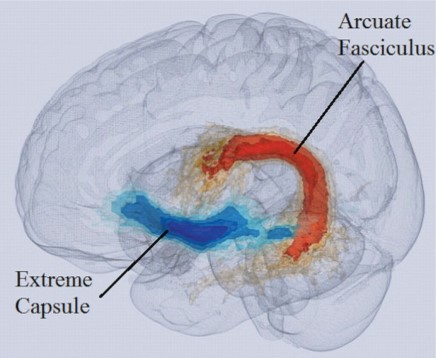
\includegraphics[scale=0.6]{cerebral_pathways.jpg}
            \end{minipage}
        \end{columns}
      \end{frame}

    \subsection{\subtwothree}
      \begin{frame}{\subtwothree}
        \begin{block}{How did we identify language centers?}
          \uncover<2->{
            The old way: disorders
            \begin{itemize}
              \item Split-brain patients
              \item Aphasias
              \begin{itemize}
                \item Broca's aphasia
                \item Wernicke's aphasia
                \item Conduction aphasia
              \end{itemize}
              \item Alexia
              \item Agraphia
            \end{itemize}
          }
        \end{block}
      \end{frame}

      \begin{frame}{\subtwothree}
        \begin{alertblock}{Split-brain patient}
          % Split brain patient
An individual who suffers from severe epilepsy who has had their corpus callosum severed as treatment

        \end{alertblock}
        \begin{block}{Evidence for lateralization}
          Split-brain patients have \href{https://youtu.be/ZMLzP1VCANo?t=96}{difficulty} naming objects that they only see with their left eye but no difficulty with the right eye
        \end{block}
        \begin{alertblock}<2->{Aphasia}
          % Aphasia
A linguistic impairment caused by damage to the brain

        \end{alertblock}
      \end{frame}

      \begin{frame}{\subtwothree}
        \begin{alertblock}{Broca's aphasia}
          % Broca's aphasia
A language impairment affecting production

        \end{alertblock}
        \begin{block}{Where might the damage be?}
          \uncover<2->{
            Broca's area
          }
        \end{block}
        \begin{example}<3->
          Can be realized as \href{https://youtu.be/JWC-cVQmEmY?t=21}{difficulty} with function words and inflections
        \end{example}
      \end{frame}

      \begin{frame}{\subtwothree}
        \begin{alertblock}{Wernicke's aphasia}
          % Wernicke's aphasia
A language impairment affecting comprehension

        \end{alertblock}
        \begin{block}{Where might the damage be?}
          \uncover<2->{
            Wernicke's area and/or the LPTJ
          }
        \end{block}
        \begin{example}<3->
          Can be realized as \href{https://youtu.be/3oef68YabD0?t=8}{difficulty} understanding others \emph{as well as} difficulty choosing semantically coherent words
        \end{example}
      \end{frame}

      \begin{frame}{\subtwothree}
        \begin{alertblock}{Conduction aphasia}
          % Conduction aphasia
A language impairment affecting a speaker's ability to produce phonologically coherent words

        \end{alertblock}
        \begin{block}{Damage area}
          Possibly the arcuate fasciculus or Wernicke's area
        \end{block}
      \end{frame}

      \begin{frame}{\subtwothree}
        \begin{block}{}
          \begin{itemize}
            \item \alert{Alexia}: % Alexia
A language impairment affecting one's ability to read

            \begin{itemize}
              \item Specifically when due to brain damage
            \end{itemize}
            \item \alert{Agraphia}: % Agraphia
A language impairment affecting one's ability to write

          \end{itemize}
        \end{block}
        \begin{block}{Damage area}
          Both result from damage to the angular gyrus
        \end{block}
      \end{frame}

    \subsection{\subtwofour}
      \begin{frame}{\subtwofour}
        \begin{block}{Try these}
          \textcite{dawson_language_2016}, chapter 9 exercises 5 and 8
        \end{block}
      \end{frame}

      \begin{frame}{References}
        \printbibliography
      \end{frame}
\end{document}
